\hypersetup{pdfborder=0 0 0}



%-------------------------------------------------------------------------------------
\section{Campagne de mesure Gibraltar 2020 (en anglais?)}
In fall 2020, field campaign in the Strait of Gibraltar (and west Alboran) aboard research and survey ship L'Atalante

\subsection{Déroulé campagne/chronologie}
%Section ce qui a ete fait pour preparer la campagne


On site measures by the ship from 8/10/2020 to 20/10/2020 . Table ... gives the period of operation and coordinate of the five moorings.


Lister les instruments...

\begin{itemize}
\item Moorings, 3 hydro (M1 M3 and M5), 2 currents (M2 and M4)  (remettre sur carte avec trace des ressauts et std Q...)
\item MVP and Seasoar profilers...
\item bathysonde equipped with niskin bottles and sensors
\item echosondeur (anglais) 3 cannaux
\end{itemize}

\begin{table}[!h]
        \centering
        \begin{tabular}{|c|c|c|}
                \hline
                M1 & N35 55.264 W005 46.739 & 8/10/2020 15h - 1/11/2020 14h\\
                M2 & N35 55.761 W005 45.288 & 8/10/2020 5h - 17/10/2020 15h\\
                M3 & N35 54.719 W005 44.459 & 8/10/2020 13h - 22/10/2020 21h\\
                M4 & N35 55.870 W005 41.020 & 8/10/2020 ?? - 17/10/2020 ??h\\
                M5 & N35 56.229 W005 41.026 & 8/10/2020 9h - 1/11/2020 14h\\
                \hline
        \end{tabular}
        %\captionof{table}{Simulation parameters}
        %\label{tab_NH-HR}
        %\end{minipage}
\end{table}


\begin{figure}[!h]
% \centering
 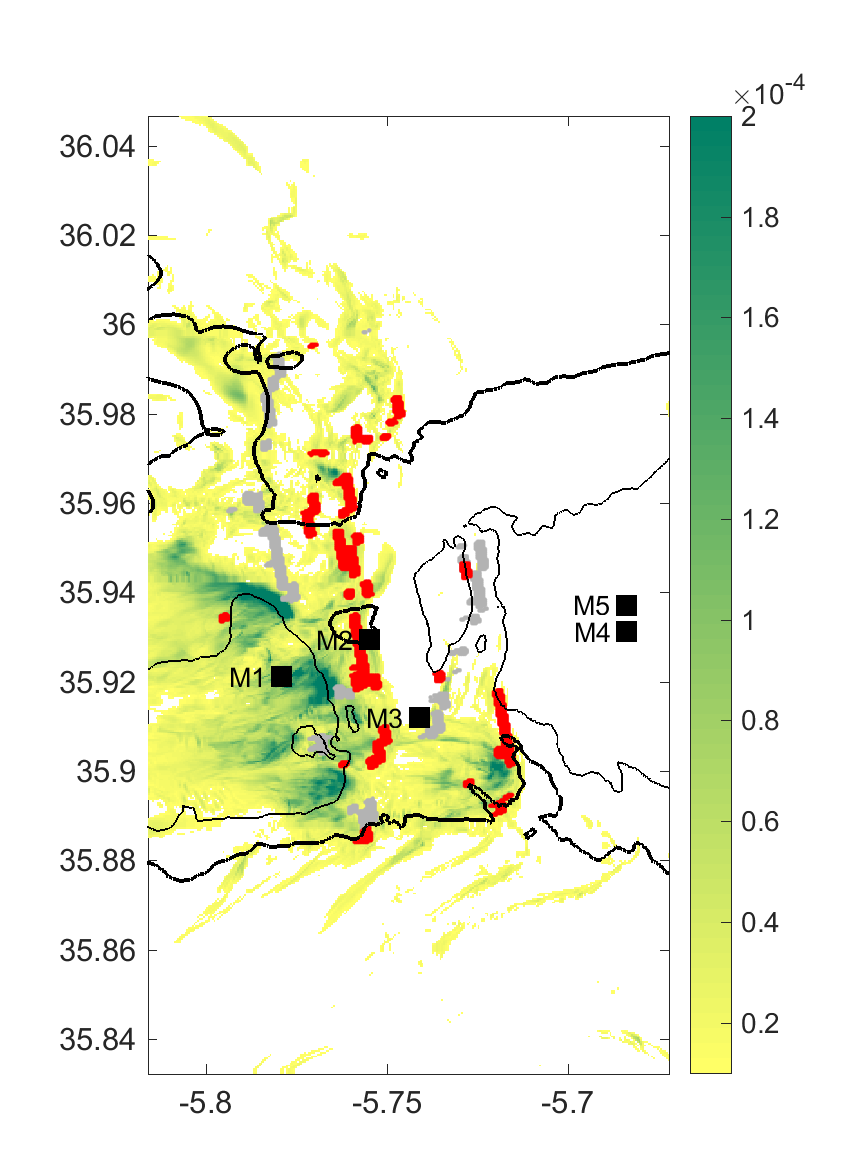
\includegraphics[width=0.4\textwidth]{./GBR3D/Fig_Moor.png}
 \caption {   }
\end{figure}


\subsection{Insights from VHR simulation}
(carte des mouillages + traces ressauts fig avant et std Q...)


\subsection{Observations of solitons}
Arrive at neap tide part of the forthnight cycle and no solitons/nor signature of hydraulic jump are observed on moorings data until 11/10/2020 



\subsection{Maquette imbriquée, comp quelques obs}

(Enleve comparaison à la maquette, pas le temps...., juste quelques obs. (ou juste a soliton, oui/non))
